\section{Užklausų klasifikacija}

Panaši problema į aptartąją įvade yra nemažai tyrinėjama duomenų bazių kontekste.
Panašiai kaip šiame darbe siekiama minimizuoti biometrinių įrašų blokų skaičių likusį po atemtimo etapo, duomenų bazėse siekiama minimizuoti disko operacijų skaičių siekiant sumažinti duomenų bazės atsako laiką bei padidinti pralaidumą (apdorotų užklausų skaičių per laiko vienetą) \cite{garcia2000database}.
Tuo tikslu yra naudojamos duomenų struktūros, vadinamos {\it duomenų indeksu}.
Jeigu duomenys yra daugiamačiai (vienas įrašas gali susidėti iš daugiau negu vienos reikšmės), tuomet indeksas tokiems duomenims vadinamas {\it daugiamačių duomenų indeksu}, o metodas pagal kurį šis indeksas yra sudaromas bei naudojamas {\it daugiamačių duomenų indeksavimo metodu}.

\subsection{Užklausų klasifikacija}

Šiame darbe palyginant biometrinių įrašų priskyrimo blokams metodus sistemoje \cite{NeurotechnologyMegamatcherAccelerator} siekiama apimti kiek galima daugiau užklausų klasių.
Gaede ir Günther \cite{gaede1998multidimensional} patiekia tokią daugiamačių užklausų klasifikaciją:
\begin{enumerate}
	\item Griežto atitikmens užklausa
	\item Taško užklausa
	\item Lango užklausa
	\item Regiono užklausa
	\item Apgaubiančioji užklausa
	\item Pilno regiono užklausa
	\item Kaimynų užklausa
	\item Artimiausio kaimyno užklausa
\end{enumerate}

Autorius duomenis ir užklausas nagrinėja $d$ dimensijų euklido erdvėje $E^d$.
Atskirus įrašus apibrėžia kaip objektus $o$ kurie gali turėti 0 ar daugiau papildomų atributų nesusijusių su erdve $E^d$ (pvz.: vardas, pavadinimas, amžius...), bei griežtai vieną atributą $o.G$, kuris apibūdina objekto $o$ padėtį erdvėje $E^d$.
Šis $o.G$ atributas yra aibė taškų, kuriuos objektas $o$ užima erdvėje $E^d$.
Objektams yra apibrėžiami operatoriai $=$, $\cap$, bei $dist(o_1, o_2)$.
Du objektai $o_1$ ir $o_2$ skaitomi lygiais $o_1 = o_2$ tada ir tik tada jeigu abiejų objektų užimamų taškų aibės $o_1.G$ ir $o_2.G$ sutampa.
Dviejų objektų $o_1$ ir $o_2$ sankirta $o_1 \cap o_2$ yra aibė taškų, kurie patenka ir į $o_1.G$ ir į $o_2.G$.
Ir galiausiai atstumas tarp dviejų objektų $o_1$ ir $o_2$ $dist(o_1, o_2)$ skaitomas atstumas tarp artimiausių taškų $p_1$, $p_2$, kur $p_1 \in o_1.G$ o $p_2 \in o_2.G$.



\subsubsection{Griežto atitikmens užklausa}
Griežto atitikmens užklausa yra tokia užklausa, kuri duotąjam objektui $o'$ erdvėje $E^d$ randa visus objektus, kurių erdvės sritys sutampa su duotąja:

\begin{equation}
	EMQ(g) = \{ o | o'.G = o.G \}
\label{eq:ExactMatchQuery}
\end{equation}

\subsubsection{Taško užklausa}
Taško užklausa yra tokia užklausa, kuri duotam taškui $p$ erdvėje $E^d$ randa visus objektus, kurie turi bendrų taškų:

\begin{equation}
	PQ(p) = \{ o | \{p\} \cap o.G = \{p\} \}
\label{eq:ExactMatchQuery}
\end{equation}

Žiūrėti priedą \ref{app:pointQuery}.

\subsubsection{Lango užklausa}
Lango užklausa, tai tokia užkausa, kuri duotiems $d$ intervalams $I^d = [l_1, u_1], [l_2, u_2], ..., [l_d, u_d]$ (po vieną intervalą kiekvienai erdvės $E^d$ koordinačių ašiai) sudaro objektą $o'$, tokį, kad

\begin{equation}
	o'.G = o'_1.G \cap o'_2.G \cap ... \cap o'_d.G
\end{equation}

Čia objekto $o'_i.G$ aibėje yra visi taškai, kurių $i$-tosios koordinatės reikšmė patenka į $I_i$ intervalą.
Lango užklausa randa visus objektus, kurie turi nors vieną bendrą tašką su objektu $o'$:

\begin{equation}
	WQ(o') = \{ o | o'.G \cap o.G \neq \emptyset \}
\label{eq:ExactMatchQuery}
\end{equation}

Verta pastebėti, kad lango užklausos atveju aibės $o'.G$ apibrėžiamos erdvės $E^d$ srities kraštinės visada yra lygegriačios šios erdvės koordinačių ašims.
Žiūrėti priedą \ref{app:windowQuery}.


\subsubsection{Regiono užklausa}
Regiono užklausa yra labai panaši į lango užklausą, tačiau $o'$ kraštinės gali būti laisvai pasirinktos ir neprivalo būti lygegriačios koordinačių ašims.
Regiono užklausa randa visus objektus, kurie turi bendrų taškų su duotuoju objektu $o'$.

\begin{equation}
	IQ(o') = \{ o | o'.G \cap o.G \neq \emptyset \}
\label{eq:ExactMatchQuery}
\end{equation}
Žiūrėti priedą \ref{app:intersectionQuery}.

\subsubsection{Apgaubiančioji užklausa}
Apgaubiančioji užklausa yra tokia užklausa, kuri randa visus objektus $o$, kurių aibė $o.G$ pilnai apima pateiktąjį objektą $o'$:

\begin{equation}
	EQ(g) = \{ o | (o'.G \cap o.G) = o.G \}
\label{eq:ExactMatchQuery}
\end{equation}
Žiūrėti priedą \ref{app:enclosureQuery}.


\subsubsection{Pilno regiono užklausa}
Pilno regiono užklausa iš esmės yra priešinga apgaubiančiąjai.
Pilno regiono užklausa yra tokia užklausa, kuri randa visus objektus $o$, kurių erdvės sritis $o.G$ pilnai patenka į pateiktajį objektą $o'$:

\begin{equation}
	CQ(g) = \{ o | (o'.G \cap o.G) = o'.G \}
\label{eq:ExactMatchQuery}
\end{equation}
Žiūrėti priedą \ref{app:containmentQuery}.


\subsubsection{Kaimynų užklausa}
Kaimynų užklausa yra tokia užklausa, kuri pagal duotąjį objektą $o'$ suranda visus šio objekto kaimynus, t.y. objektus $o$ kurie turi bendrą kraštinę erdvėje $E^d$:

\begin{equation}
	AQ(g) = \{ o | (o'.G \cap o.G) \neq \emptyset \land o'.G\textdegree \cap o.G\textdegree = \emptyset \}
\label{eq:ExactMatchQuery}
\end{equation}

Čia $o.G\textdegree$ reiškia visus vidinius taškus, kurie priklauso aibei $o.G$.
Vidiniais taškais skaitomi tie taškai, kurie nepakliūna ant objekto $o$ apibrėžiamos erdvės srities kraštinių.
Žiūrėti priedą \ref{app:adjacencyQuery}.


\subsubsection{Artimiausio kaimyno užklausa}
Artimiausio kaimyno užklausa yra tokia užklausa, kuri duotam objektui $o'$ randa artimiausią kaimyną (verta pastebėti, kad šiuo atveju kaimynai gali ir neturėti bendrų kraštinių).

\begin{equation}
	NNQ(o') = \{ o | \forall o'' : dist(o'.G, o.G) \leq dist(o'.G, o''.G) \}
\label{eq:ExactMatchQuery}
\end{equation}




\section{Daugiamačių duomenų indeksavimo metodų klasifikacija}
Lu ir Ooi \cite{lu1993spatial}, Gaede ir Günther \cite{gaede1998multidimensional}, bei B{\"o}hm, Christian, Stefan, Daniel A \cite{bohm2001searching} apžvelgia įvairius daugiamačių duomenų indeksus, bei pateikia schemą padedančią suprasti jų istoriją (žiūrėti priedą \ref{app:multidimensionalIndexing}).

Autoriai šiuos metodus suskirsto į tris grupes:
\begin{itemize}
	\item Metodai paremti maišos funkcijomis.
	\item Hierarchiniai metodai.
	\item Metodai paremti erdvę užpildančiomis kreivėmis \cite{bader2012space}.
\end{itemize}



\subsection{Maišos funkcijomis paremti metodai daugiamačių duomenų indeksavimui}

Bendruoju atveju maišos funkcijomis paremti metodai yra tinkami griežto atitinkmens, bei taško užklausoms.
Tačiau siekiant apdoroti lango, regiono ir kitas, panašias, užklausias šie metodai tampa kompleksiškesni \cite{nievergelt1981grid} \cite{tamminen1982excell}.
Dėl šios priežasties jie nebus nagrinėjami, įgyvendinami ir lyginami šiame darbe.


\subsection{Hierarchiniai metodai daugiamačių duomenų indeksavimui}
\label{sec:HierarchicalIndices}

Hierarchiniai daugiamačių duomenų indeksai yra paremti dvejetainiais ar aukštesnio atsišakojimo laipsnio medžiais (trejetainiai, ketvirtainiai...) \cite{gaede1998multidimensional}.
Šie indeksai saugo įrašus ne po vieną, bet grupėmis.
Dažniausiai kiekviena grupė yra randama medžio lapuose (vadinama {\it duomenų viršūne}).
Vidinės viršūnės (vadinamos {\it indekso viršūnėmis}) yra naudojamos kaip kelrodžiai ieškant duomenų viršūnių.
Kiekviena indekso viršūnė nurodo visas duomenų viršūnes, kurios gali būti rastos šios indekso viršūnės pomedyje.

Keletas tokių medžių pavyzdžių yra R-medis \cite{guttman1984r}, R*-medis \cite{beckmann1990r}, R+-medis \cite{sellis1987r+}, Kd-medis \cite{bentley1979multidimensional}, Kdb-medis \cite{robinson1981kdb}, X-medis \cite{berchtold1996x}, Quad-medis \cite{habenicht1983quad} ir daug kitų.

Užklausų apdorojimas yra skaidomas į du etapus \cite{bohm2001searching}:
\begin{enumerate}
	\item Iteravimas medžiu.
	\item Įrašų filtravimas.
\end{enumerate}
Iteravimo medžiu etape, yra „prabėgamas“ medis nuo šaknies iki lapų ir atrenkamos visos duomenų viršūnės, kurios gali turėti įrašų atitinkančių užklausą.
Filtravimo metu atrenkami įrašai esantys iteravimo etape atrinktose duomenų viršūnėse ir tenkinatys užklausą \cite{brinkhoff1994multi} \cite{bohm2001searching}.
Verta pastebėti, kad sistemoje \cite{NeurotechnologyMegamatcherAccelerator} užklausų apdorojimo etapai yra labai panašūs.

\paragraph{Kd-medis}
\label{sec:Kd-tree}

Šiame darbe bus aptariamas biometrinių įrašų priskyrimo blokams metodas paremtas Kd-medžiu \cite{bentley1979multidimensional}.
Kd-medis yra dvejetainis medis, kurio lapuose (duomenų viršūnėse) yra saugomi vienas ar daugiau $d$-mačių taškų.
Kiekviena vidinė medžio viršūnė (indekso viršūnė) dalina erdvę $E^d$ į dvi nepersidengiančias dalis.
Taškai patenkantys į vieną dalį patenka į kairyjį pomedį, o patenkantis į kitą dalį -- į dešinį pomedį (žr.: \ref{img:KdTreeExample} pav.).
Erdvės dalinimas į dvi dalis yra parenkamas taip: kiekvienai indekso viršūnei yra parenkama koordinačių ašis (pvz.: $x$) ir reikšmė (pvz .: $5$).
Tuomet visi taškai, kurių $x$ koordinatės reikšmė yra mažesnė už parinktą reikšmę (pavyzdyje $[-\infty; 5)$), patenka į kairyjį pomedį, o likę taškai (pavyzdyje $[5; \infty)$) -- į dešinį pomedį.
Nėra griežtai apibrėžta kokia koordinačių ašis ar reikšmė šioje ašyje turi būti parinkta kiekvienai viršūnei, todėl šiuo tikslu taikomos įvairios euristikos.

\begin{figure}[H]
\begin{center}
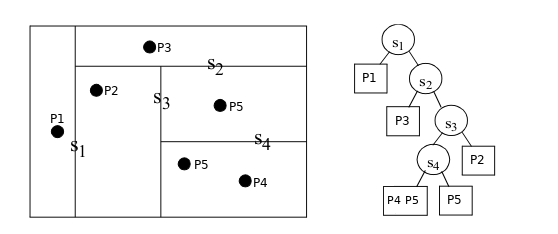
\includegraphics[width=0.7\textwidth]{img/KdTreeExample.png}
\caption{Kd-medžio pavyzdys.}
\label{img:KdTreeExample}
\end{center}
\end{figure}

Paveiksliuke \ref{img:KdTreeExample} pateikiamas Kd-medžio pavyzdys.
Čia kairėje -- šį medį atitinkanti erdvė $E^d$.
Taškai $P1$-$P5$ atitinka daugiamačius duomenis, o tiesės $S1$-$S4$ - erdvės $E^d$ padalijimus atitinkmai medžio viršūnėse $S1$ - $S4$.

Hierarchiniai metodai daugiamačių duomenų indeksavimui yra plačiai taikomi duomenų bazių \cite{bohm2001searching}, sensorių tinklų \cite{li2003multi}, paveiksliukų paieškoje \cite{silpa2008optimised}, privatumo \cite{hore2012secure} \cite{xiao2010differentially} ir kitose srityse.

\subsection{Erdvę užpildančiomis kreivėmis paremti metodai daugiamačių duomenų indeksavimui}

Kaip ir hierarchiniuose metoduose taip ir erdvę užpildančiomis kreivėmis paremtuose metoduose duomenys nagrinėjami kaip taškai d-matėje erdvėje $E^d$.

Daugiamačiai duomenys neturi pilnos tvarkos, pagal kurią šalia esantys taškai būtų arti ir erdvėje $E^d$.
Dėl šios priežasties daugiamačių duomenų indeksavimo metodai yra sudėtingesni lyginant su vienmačiais \cite{gaede1998multidimensional} \cite{bohm2001searching}
Tačiau egzistuoja įvairiomis euristikomis paremtų pilnos tvarkos sudarymo metodų, kurie su tam tikra tikimybe taip sudeda taškus.
Surikiavus taškus pagal šią pilną tvarką juos galima indeksuoti vienmačiais indeksavimo metodais (B-medžiu \cite{comer1979ubiquitous} RB-medžiu \cite{hanke1997relaxed} ir pan.).

Siekiant sudaryti tokią tvarką, $E^d$ erdvė suskirstoma į gardelę (į kiekvieną laukelį šioje gardelėje gali patekti nulis, vienas ar daugiau taškų).
Kiekvienam laukeliui šioje gardelėje yra priskiriamas unikalus skaičius pagal kurį laukeliai yra surikiuojami ir indeksuojami vienmačiais indeksavimo metodais.
Šie unikalūs skaičiai yra priskiriami pagal tvarką, kuria erdvę užpildanti kreivė „prabėga“ pro laukelius \cite{bader2012space}.
Aptarsime dvi tokias kreives:
\begin{enumerate}
	\item Eilutinę kreivę.
	\item Z-kreivę.
\end{enumerate}

\paragraph{Eilutinė kreivė}

Eilutinė kreivė yra viena iš papraščiausių erdvę užpildančių kreivių.
Ji negali būti naudojama begalinėje erdvėje, todėl tarkime, kad $[L_i, U_i]$ yra erdvės $E^d$ ribos koordinačių ašies $i$ atžvilgiu.
Eilutinė kreivė iš pradžių „prabėga“ visus taškus $[x, L_2, ..., L_d]$, kur $x$ patenka į intervalą $[L_1, U_1]$.
Šis prabėgimas atliekamas $x$ didėjimo tvarka.
Paskui „prabėga“ $[x, L_2 + 1, ..., L_d]$, paskui $[x, L_2 + 2, ..., L_d]$ ir t.t. (žr.: \ref{img:RowWiseSpaceFillingCurve} pav.).

\begin{figure}[H]
\begin{center}
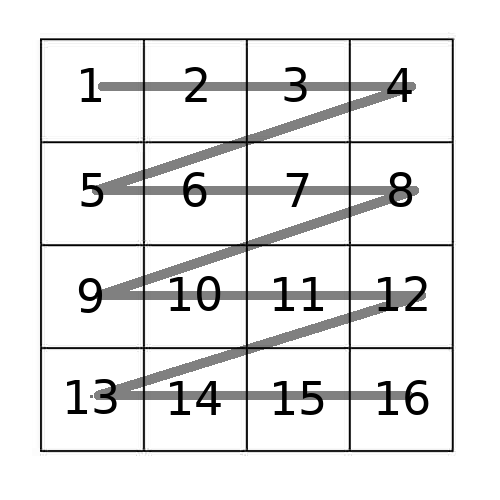
\includegraphics[width=0.3\textwidth]{img/RowWiseSpaceFillingCurve.png}
\caption{Eilutinės erdvę užpildančios kreivės pavyzdys.}
\label{img:RowWiseSpaceFillingCurve}
\end{center}
\end{figure}


Formaliai pilna tvarka yra apibrėžiama sąryšio:
\begin{equation}
	p_1 < p_2 \text{ jeigu } RWSFC(p_1) < RWSFC(p_2)
\label{eq:RowWiseSFCComparison}
\end{equation}

Čia $p_1$ ir $p_2$ yra taškai erdvėje $E^d$, o $RWSFC(p)$:

\begin{equation}
	RWSFC(p) = 1 + \sum_{i=1}^{d} [(p_i - L_i) \prod_{j=0}^{i - 1}U_j - L_j]
\label{eq:RowWiseSFCValue}
\end{equation}

Čia daroma prielaida, kad $U_0 - L_0 = 1$.



\paragraph{Z-kreivė}

Z-kreivė daugiamačių duomenų indeksavimo metodų, paremtų erdvę užpildančiomis kreivėmis, kontekste yra viena iš populiariausių \cite{ramsak2000integrating}.
Z-kreivė visų pirma visą erdvę $E^d$ padalina į dvi lygias sritis $P_0$ ir $P_1$ statmenai pirmai koordinačių ašiai.
Visi laukeliai esantys srityje $P_0$ yra pirmiau tų, kurie yra srityje $P_1$.
Sekančiame žingsnyje $P_0$ yra padaliniama į dvi lygias sritis $P_{00}$, $P_{01}$, o $P_1$ yra padalinama $P_{10}$ $P_{11}$ statmenai antrai koordinačių ašiai.
Atitinkamai $P_{00}$ laukeliai yra pirmesni už $P_{01}$, o $P_{10}$ pirmesni už $P_{11}$.
Toliau skaidoma pagal trečią koordinačių ašį, vėliau pagal ketvirtą, ..., d-tąją (žr.: \ref{img:ZCurveSpaceFillingCurve} pav.).
Kai padaromas padalinimas pagal d-tąją ašį, pradedama vėl nuo pirmosios koordinačių ašies.
Šis rekursiškas dalinimas yra vykdomas tol, kol kiekviena erdvės sritis $P$ yra nedidesnė negu ankščiau minėtos gardelės laukelio dydis.

\begin{figure}[H]
\begin{center}
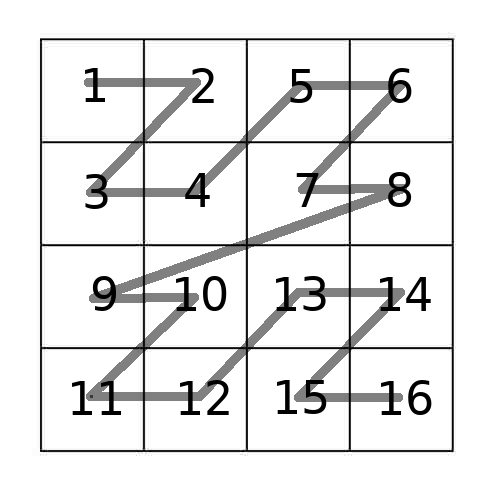
\includegraphics[width=0.3\textwidth]{img/ZCurveSpaceFillingCurve.png}
\caption{Z erdvę užpildančios kreivės pavyzdys.}
\label{img:ZCurveSpaceFillingCurve}
\end{center}
\end{figure}

Tarsime, kad erdvė $E^d$ nėra begalinė, ir $[0, 2^b]$ yra visų šios erdvės koordinačių ašių ribos.
Formaliai tvarka yra apibrėžiama sąryšio:
\begin{equation}
	p_1 < p_2 \text{ jeigu } ZCSFC(p_1) < ZCSFC(p_2)
\label{eq:ZCurveSFCComparison}
\end{equation}

Čia $p_1$ ir $p_2$ yra taškai erdvėje $E^d$, o $ZCSFC(p)$:

\begin{equation}
	ZCSFC(p) = 1 + \sum_{i=0}^{b-1} \sum_{j=0}^{d-1} [2^{i*b+j} BITSET(p_j, i)]
\label{eq:ZCurveSFCValue}
\end{equation}


\begin{equation}
	BITSET(p, i)=
\begin{cases}
	1,& \text{jeigu } \text{i-asis bitas yra 1 skaičiaus p dvejetainėje formoje}\\
	0,& \text{kitu atveju}\\
\end{cases}
\label{eq:Bitset}
\end{equation}






\section{SP-GIST karkasas}

Walid G. Aref, Ihab F. Ilyas \cite{aref2001sp} pastebėjo, kad siekiant įdiegti ar palyginti įvairius hierarchinius duomenų indeksavimo metodus tenka kiekvieną jų atskirai integruoti į duomenų bazės branduolį.
Tai yra sudėtinga ir daug laiko reikalaujanti užduotis.
Autoriai šią problemą sprendė ieškodami bendrų savybių visiems hierarchiniams duomenų indeksavimo metodams ir pasiūlė sąsają, kuri galėtų būti integruota į duomenų bazės branduolį.
Suprogramuoti indeksavimo metodą pagal šią sąsaja yra kur kas lengvesnė užduotis, negu integruoti tiesiai į duomenų bazės branduolį.
Verta pastebėti, kad tokia pati problema panašiu būdu buvo spręsta ir vienmačių duomenų indeksavimo metodams \cite{hellerstein1995generalized}.

Autorių pasiūlyta SP-GIST sąsaja susideda iš 7 parametrų ir 3 metodų.
Naudodamasis šiais parametrais ir metodais duomenų bazės branduolys gali išsaugoti, ištrinti įrašus bei apdoroti užklausas.

\subsection{SP-GIST sąsajos parametrai}
Tokie parametrai yra apibrėžiami autorių (pateikiami originalo kalba):
\begin{enumerate}
	\item NodePredicate.
	\item KeyType.
	\item NumberOfSpacePartitions.
	\item Resolution.
	\item PathShrink.
	\item NodeShrink.
	\item BucketSize.
\end{enumerate}

Trumpai aptarsime šiuos parametrus.

\paragraph{NodePredicate}
Parametras {\it NodePredicate} apibrėžia duomenų struktūrą, kuri yra saugoma indekso viršūnėse.
Pagal šiuos duomenis yra parenkamas indekso viršūnės vaikas, pro kurį bus iteruojama toliau.
Pavyzdžiui Kd-medžio atveju šis parametras apibrėžtų duomenų tipą saugantį koordinačių ašį ir reikšmę, pagal kurią indekso viršūnėje dalijama erdvė $E^d$ (žr.: \ref{sec:Kd-tree} skyrelį).

\paragraph{KeyType}
Parametras {\it KeyType} nurodo kokio tipo duomenys yra saugomi duomenų viršūnėse.
Šiame darbe nagrinėsime tik tuos atvejus, kur šio parametro reikšmė yra taškų erdvėje $E^d$ aibė.

\paragraph{NumberOfSpacePartitions}
Parametras {\it NumberOfSpacePartitions} apibrėžia kiek daugiausiai vaikų gali turėti indekso viršūnės.
Pavyzdžiui Kd-medžio atveju šio parametro reikšmė yra $2$, quad-medžio atveju -- $4$.

\paragraph{Resolution}
Parametras {\it Resolution} apibrėžia maksimalų medžio gylį.

\paragraph{PathShrink}
Parametras {\it PathShrink} gali turėti tris reikšmes: {\it NeverShrink}, {\it LeafShrink} arba {\it Tree Shrink}.
Kai kuriais atvejais hierarchiniuose duomenų indeksavimo metoduose dvi ar daugiau indekso viršunių gali būti apjungtos tarpusavyje, šitaip sumažinant medžio gylį, tačiau neprarandant duomenų vientisumo.
Tačiau šiame darbe šie apjungimo metodai nebus nagrinėjami ir bus daroma prielaida, kad parametro {\it PathSrhink} reikšmė visada bus {\it NeverShrink}, t.y. niekada nebus vykdomi indekso viršūnių apjungimai.

\paragraph{NodeShrink}
Verta prisiminti, kad hierarchiniai duomenų indeksavimo metodai duomenis laiko grupėmis (žr.: \ref{sec:HierarchicalIndices}).
Parametras {\it NodeShrink} gali turėti dvi reikšmes: „Įjungta“ arba „Išjungta“.
Jeigu reikšmė yra „Įjungta“, tuomet tuščios duomenų viršūnės (pavyzdžiui po visų įrašų priklausančių kuriai nors duomenų viršūnei ištrynimo) bus pašalinamos iš medžio.
Atitinkamai, jeigu indekso viršūnė nebeturi vaikų -- ji irgi bus pašalinta.
Jeigu reikšmė yra „Išjungta“, tuščios viršūnės yra paliekamos medyje.


\paragraph{BucketSize}
{\it BucketSize} parametras nurodo kiek daugiausiai įrašų gali būti vienoje duomenų viršūnėje (grupėje).



\subsection{SP-GIST sąsajos metodai}

Autoriai apibrėžė šiuos metodus SP-GIST sąsajoje (pateikiami originalo kalba):
\begin{enumerate}
	\item {\it Consistent(Entry E, Query q)}
	\item {\it PickSplit(P)}
	\item {\it Cluster()}
\end{enumerate}

\paragraph{Metodas Consistent}
Metodas {\it Consistent(Entry E, Query q)} yra būlio funkcija, kuri gražina rezultatą {\it Melas} tada ir tik tada, jeigu viršūnėje $E$ (ir jos pomedyje jeigu viršūnė $E$ yra indekso viršūnė) negali būti įrašų, kurie tenkina užklausą $q$.
Šis metodas yra naudojamas duomenų bazės branduolio kaip kelrodis iteruojant per medį.

\paragraph{Metodas PickSplit}
Jeigu duomenų viršūnėje, į kurią bandoma įdėti naują įrašą, nebėra laisvos vietos (įrašų skaičius joje pasiekė parametro {\it BucketSize} reikšmę), tuomet ši viršūnė yra skaidoma į dvi ar daugiau naujų viršūnių.
Metodas {\it PickSplit(P)} yra naudojamas siekiant parinkti kaip duomenų viršūnė $P$ pasidalins į mažesnes.
Šis metodas gražina medį, saugantį visus įrašus buvusius viršūnėje $P$.
Duomenų bazės branduolys, duomenų viršūnę $P$, pakeičia gražinto medžio šaknine viršūne.

\paragraph{Metodas Cluster}
Metodas {\it Cluster()} parenka kaip medžio viršūnės bus saugomos disko blokuose.
Kadangi šiame darbe nagrinėjame indeksus, kurie saugo įrašus operatyviojoje atmintyje, tai šis metodas nebus detalizuojamas.

Šis karkasas yra naudojamas populiariose duomenų bazėse \cite{eltabakh2006space}.
Taip pat modifikuota (konkrečios modifikacijos aprašomos sekančiuose skyreliuose) ši sąsaja bus taikoma ir vertinant biometrinių įrašų priskyrimo blokams metodus paremtus ir Kd-medžiu ir erdvę užpildančiomis kreivėmis sistemoje \cite{NeurotechnologyMegamatcherAccelerator}.


